% 
% Application
% @author Pieter Maene <pieter.maene@student.kuleuven.be>
%

\section{Application}

The modified Helios voting system was used in the elections for the new board of VTK. This is the official student organisation for engineering students at the KU Leuven. First, support for some new features had to be added. The system was then thoroughly tested before the election on May 8\textsuperscript{th} 2014.

\subsection{Adjustments}

Shibboleth is the single sign-on system used by the KU Leuven. Students have an account with a unique identification number. All voters in the election have such an account, so it could be used to authenticate them. Since Helios' authentication system is modular and already has support for other federated identity systems, adding Shibboleth was relatively straightforward.

\par The list of voters was provided by an external organisation. This included the student's identification number and name, but his e-mail address was missing. This is needed by Helios to send a confirmation message after casting a ballot. A voter's student e-mail address is retrieved from the Shibboleth response and added to his account to fix this.

\par Helios did not yet show the election's participation percentage. This is the percentage of eligible voters that cast their vote. The system also immediately published the election result. They are traditionally announced to the public at midnight, but the election administrator does need earlier access to them. These two smaller features were therefore implemented as well.

\subsection{Tests}

After installing the system on a server, it was thoroughly tested. In addition to verifying all technical aspects, the testers were also asked for feedback on the user interfaces. The election admin and booth were tested in the context of the actual election. The real voter list was replaced by the current board of the organisation, though.

\par While testing the threshold encryption process, a bug was found. Real fractions were used for the calculation of the Lagrange interpolation, instead of finite modular arithmetic. After solving this, the result still couldn't be decrypted correctly. By default, Helios was added as a trustee to the election. It completed all steps in the ceremony automatically. During testing, the shares of this trustee turned out to be incompatible with these generated by the other trustees. The only difference between the two is that the former are generated in the Python application and the latter in the JavaScript trustee dashboard. Because the error could not be found, Helios no longer could be an election trustee. Since its role in the whole process was already limited, this was not a big change. The main advantage of adding it, was that it allowed users to create an election without real trustees, which resulted in a simpler procedure.

\par Apart from these bugs, the test of the election admin went very well. The election administrator managed to go through the entire procedure independently. The trustees didn't have much difficulty generating their keys either.

\par Although its functionality worked perfectly, a lot of feedback was given on the voting booth. First, a lot of technical terms were used. This was easily solved by replacing them with more common words. Second, most testers found the voting process to be too complicated. The booth is an independent application written in JavaScript, so that only the encrypted vote is sent to the server.

\par There were two places where the user had to submit his vote originally. After confirming his encrypted vote in the booth (\ref{fig:app:booth_submit}), it was sent to the server where it could finally be cast. The last screen of the voting booth was therefore removed. Since it still had to be possible to audit the encrypted vote, this also required the encryption to be moved. This is now done after the voter has made all his choices. As a result, the vote has to be re-encrypted when these are changed. The current implementation is already reasonably fast and this will only improve once the Web Cryptography API is available (\ref{sec:web_cryptography_api}). The test was repeated after making these adjustments to verify their impact on both functionality and usability.

\begin{figure}
  \center{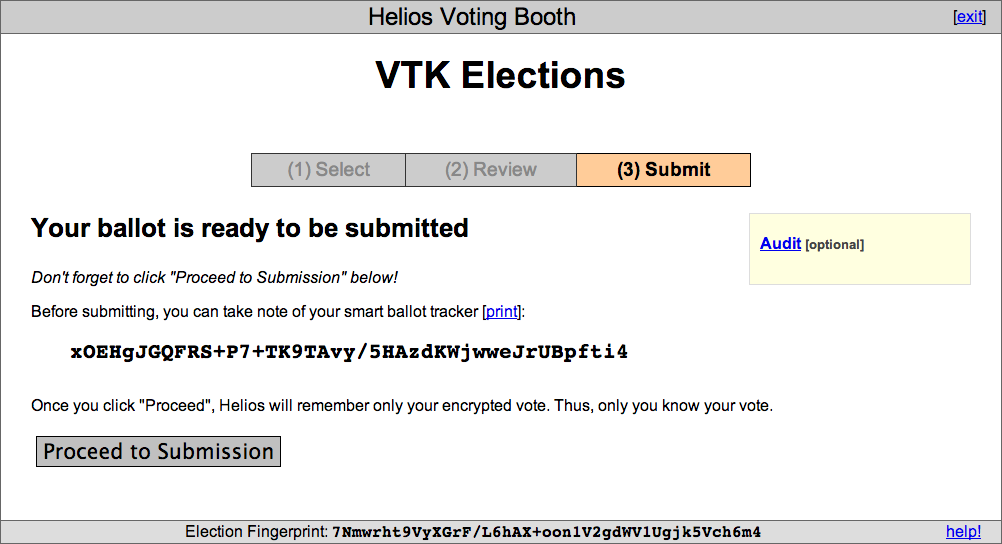
\includegraphics[width=\linewidth]{booth_submit.png}}
  \caption{Last Screen of the Voting Booth}
  \label{fig:app:booth_submit}
\end{figure}

\par Finally, a stress test was run as well. This was done for a separate election with two trustees and three questions. \np{1000} votes were inserted into the database. To do this, the encrypted votes were generated directly in Python instead of using the JavaScript voting booth. The result was decrypted successfully, indicating that the system can manage an election of that size.

\subsection{Election Day}

The election itself took place on May 8\textsuperscript{th} 2014 from 7 am till 8 pm. During this time, 768 people cast a ballot which isn't significantly less than during previous years. This is a strong indication that the voting process was clear.

\par Since everything had been tested in advance, no problems were encountered during the voting or when decrypting the result.
